% Page format
\documentclass[a4paper,12pt]{article}

\usepackage[utf8]{inputenc}
\usepackage{geometry}
\geometry{
    a4paper,
    total={170mm,257mm},
    left=20mm,
    top=20mm,
}

% Font type
\usepackage{DejaVuSans}
\renewcommand*\familydefault{\sfdefault}
\usepackage[T1]{fontenc}

\usepackage{parskip}

\usepackage[spanish, galician]{babel}

\usepackage{rotating}\usepackage{float}

% use adjustwit to group margin
\usepackage{changepage}

% sectional headers size
\usepackage{titlesec}

% Font size
\usepackage[12pt]{moresize}


% Double space
\setlength{\parskip}{1em}
\setlength\headheight{15pt}
\renewcommand{\baselinestretch}{1.5}



% Cover Border
\usepackage{tikz}
\usetikzlibrary{calc}

\usepackage{graphicx}
\graphicspath{ {images/} }


% Links format
\usepackage{hyperref}
\hypersetup{
    colorlinks=true,
    linkcolor=blue,
    filecolor=magenta,      
    urlcolor=blue,
    pdftitle={Overleaf Example},
    pdfpagemode=FullScreen,
    }
% notes  
\usepackage{marginnote}

% tables
\usepackage{multirow}

% list
\usepackage{enumitem}

\usepackage{verbatimbox}

% Header & footer page
\usepackage{fancyhdr}
\pagestyle{fancy}
\usepackage{lastpage}

\renewcommand{\footrulewidth}{0.3pt}

% anula la interpretación de comillas y dieresis
\renewcommand{\shorthandsspanish}{}


% CONTENT

% VARIABLES
\def\curso{Desenvolvemento de Aplicacións Multimedia (DAM)}
\def\asignatura{MP0485. Programación.}
\def\ud{Unidad 1}
\def\titulo{INTRODUCCIÓN A LA\\
 PROGRAMACIÓN ESTRUCTURADA}
\def\titulotiny{PROG-UD1: Prog. Estructurada}
\def\numTarea{PROG1}
\def\filename{Martinez\_Costas\_Rafael\_PROG\_ProgEstruct\_Tarea.pdf}
\def\dateCreation{12 de octubre do 2023}
\def\estudiante{Rafael Martínez Costas (Grupo B)}
\begin{document}
% --------------------------------------
% ---------  COVER ---------------------
% --------------------------------------

\begin{titlepage}

      % Border
      \begin{tikzpicture}[overlay,remember picture]
            \draw
            ($ (current page.north west) + (1.5cm,-1.5cm) $)
            rectangle
            ($ (current page.south east) + (-1.5cm,1.5cm) $);

      \end{tikzpicture}

      \vspace{-0.7 cm}
      % header of cover
      \large \curso

      \vspace{-0.5 cm}
      \large\textbf{\asignatura}

      % main title
      \rule{17cm}{0.5mm}
      \Large\textbf{\ud}
      \vspace{-0.5 cm}

      \huge\textcolor{lightgray}{\textbf{\titulo}}

      \vspace{0.6 cm}

      \large\textbf{\filename}

      \vspace{-0.8 cm}

      \rule{17cm}{0.5mm}

      \Large \dateCreation

      \vspace{11.6cm}
      \rule{17cm}{0.5mm}

      \vspace{-0.6 cm}
      \begin{flushright}
            \normalsize Estudiante:
            \normalsize\textbf{\estudiante}
      \end{flushright}

\end{titlepage}


\linespread{1.5}

\section{Tarea \numTarea}
% --------------------------------------
% ---------  Actividad 1 ---------------
% --------------------------------------
\subsection{Código}
En las soluciones de los otros ejercicios cada entrada individual tiene su salida,
pero según pone el enunciado, parece que todas las entradas se escriben a la vez y,
después, se muestra la salida.
En mi caso lo hice de esa forma.

\begin{verbnobox}[\fontsize{12pt}{12pt}\selectfont]
/* Ejercicio a enviar de EV1
    Fin de mes
 */
fun main() {
    // print("Introduce casos a probar: ")
    val casos = readln().toInt()
    val primerDia =  IntArray(casos)
    val cambio = IntArray(casos)

    // PEDIMOS DATOS
    for(i in 0 until casos){
        // print("Introduce \"Saldo primer día mes\" y el \"cambio estimado\": ")
        val input = readln().split(" ")
        primerDia[i] = input[0].toInt()
        cambio[i] = input[1].toInt()
    }

    // MOSTRAMOS RESULTADO
    for(i in 0 until casos){
        if(primerDia[i] + cambio[i] < 0){
            println("NO")
        }else{
            println("SÍ")
        }
    }
}
\end{verbnobox}
\clearpage
\subsection{Funcionamiento}
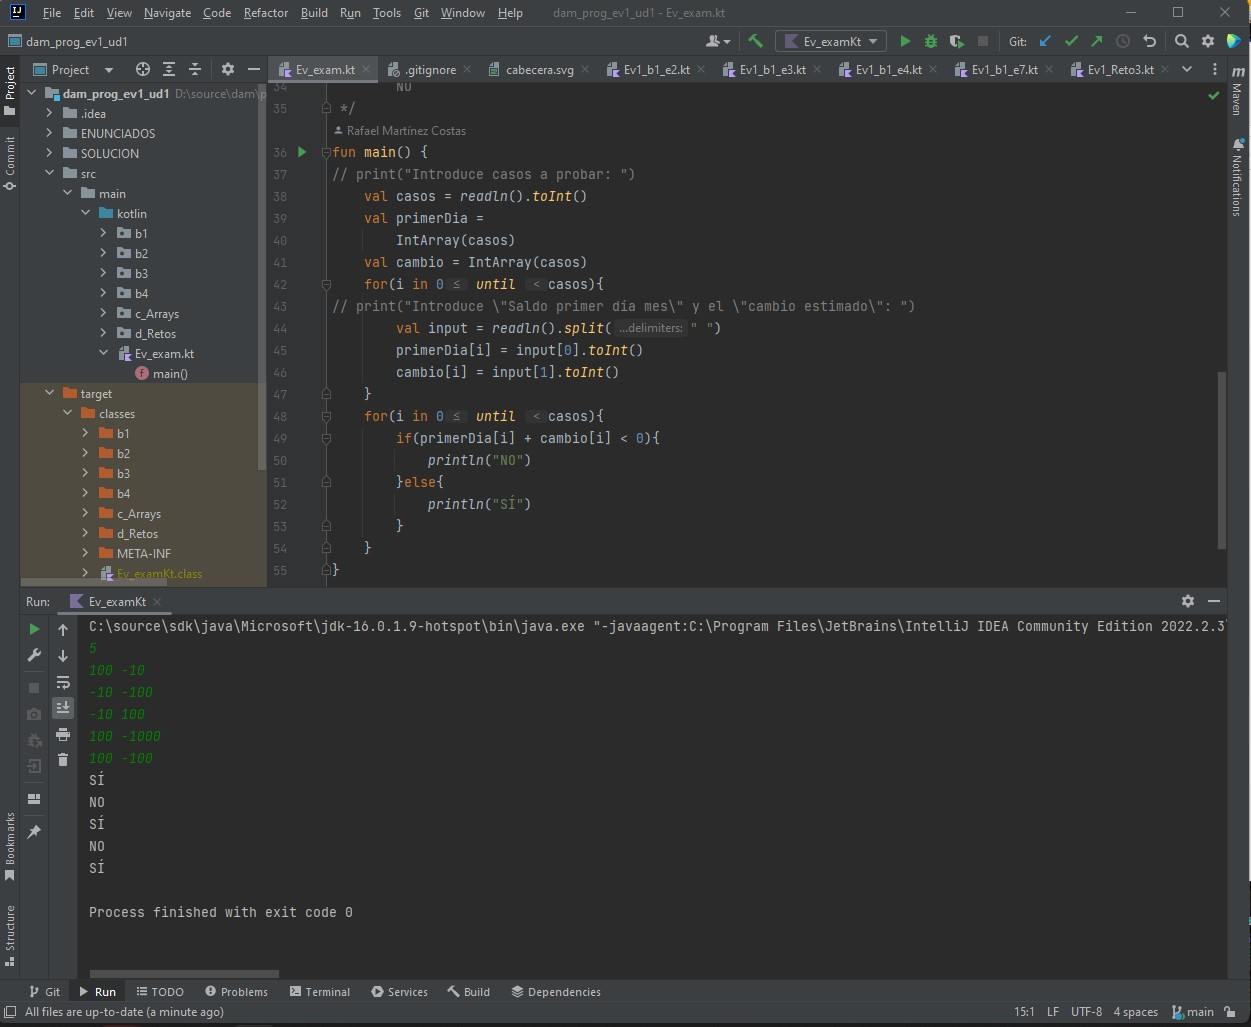
\includegraphics[width=17cm]{Captura}
\end{document}
\phantomsection
